\renewcommand{\appref}[1]{, c.f. Appendix, Def.\,\ref{#1}}
 
%As was have seen, \Chainmail assertions not only talk about the contents of the current state (stack frame and heap),
%but they also talk about future and past states, Therefore, 
The meaning of \Chainmail assertions is parametric with an
underlying object-oriented programming language, with modules  as repositories of code, classes with fields, methods and
ghostfields, objects described by classes, a way to link  modules into larger ones, and a concept of 
program execution.\footnote{We believe that \Chainmail can be applied to 
any language with these features.}

We have developed   \LangOO, a minimal such object-oriented language, which we
outline in  this section. 
We  describe the novel aspects of \LangOO,, and 
summarise the more conventional parts, relegating  full, and mostly unsurprising,
definitions %for  \LangOO~appear 
to Appendix \ref{app:LangOO},  
 

Modules are central to \LangOO, as they are to \Chainmail. As modules are repositories
of code, we adopt the common formalisation of modules as maps from 
class identifiers to class definitions\appref{defONE}. We use the terms module and component in an
analogous manner to class and object respectively. Class
definitions consist of field, method and ghost field declarations\appref{def:syntax:classes}.  \LangOO is untyped -- this reflects the
open world, where we link with external modules which come without any
guarantees.
Method bodies are sequences of 
statements, which  can be field read or field assignments, object
creation, method calls, and return statements. 
%All else, \eg booleans, conditionals, loops,  can be encoded.
Fields are private in the sense of C++: they can only be read or
written by methods of the current class.
This is enforced by the operational semantics, \cf Fig.  \ref{fig:Execution}.
We  discuss ghost fields in the next section.

Runtime configurations, $\sigma$,  contain   all the usual information about an execution snapshot: the heap, and a
stack of frames. The code to be executed is kept as part of the runtime configuration:
%
Each frame consists of a continuation, \prg{contn}, describing the remaining code to be executed by the
frame, and a map from
variables to values. Values are either addresses or sets of addresses; the latter 
are needed to deal with assertions which quantify over sets of objects, as
\eg (1) and (2) from section \ref{sect:motivate:Bank}.
% 
We define {\emph{one-module} execution  through a judgment of the form $\M, \sigma \leadsto \sigma'$ in the Appendix, Fig.  \ref{fig:Execution}. 
%
  

We define a module linking operator \  $\link$ \  so that
$\M\link\M'$ is the union of the two modules, provided that their domains are disjoint\appref{def:link}.
 %
As we said in section \ref{sect:overviewmodel}, we distinguish  between the internal and external module, and treat  execution of 
methods from the internal module as atomic. For this, we define \emph{two-module execution}  based on
one-module execution as follows:

%Susan: I don't understand this when n = 2
\begin{definition}
\label{def:execution:internal:external}
\label{def:module_pair_execution} 
Given runtime configurations $\sigma$,  $\sigma'$,  and a module-pair $\M \mkpair \M'$ we define
execution where $\M$ is the internal, and $\M'$ is the external module as below:
 
\begin{itemize}
\item
$\M \mkpair \M', \sigma \leadsto \sigma'$ \IFF
there exist  $n\geq 2$ and runtime configurations $\sigma_1$,  ...
$\sigma_n$, such that
\begin{itemize}
\item
$\sigma$=$\sigma_1$,\ \  \ \ and\ \ \ \ $\sigma_n=\sigma'$.
\item
$\M \link \M', \sigma_i \leadsto \sigma_{i+1}'$,\  \  for $1\leq i \leq n\!-\!1$
\item
$\ClassOf{\this} {\sigma}\not\in dom({\M})$,  \ \  \ \ and\ \ \ \
$\ClassOf{\this} {\sigma'} \not\in dom({\M})$,
\item
 $\ClassOf{\this} {\sigma_i} \in dom({\M})$,\ \ \ \ for $2\leq i \leq n\!-\!2$
\end{itemize}
\end{itemize}

\end{definition}

 \begin{figure}[htb]
 \begin{minipage}{0.80\textwidth}
 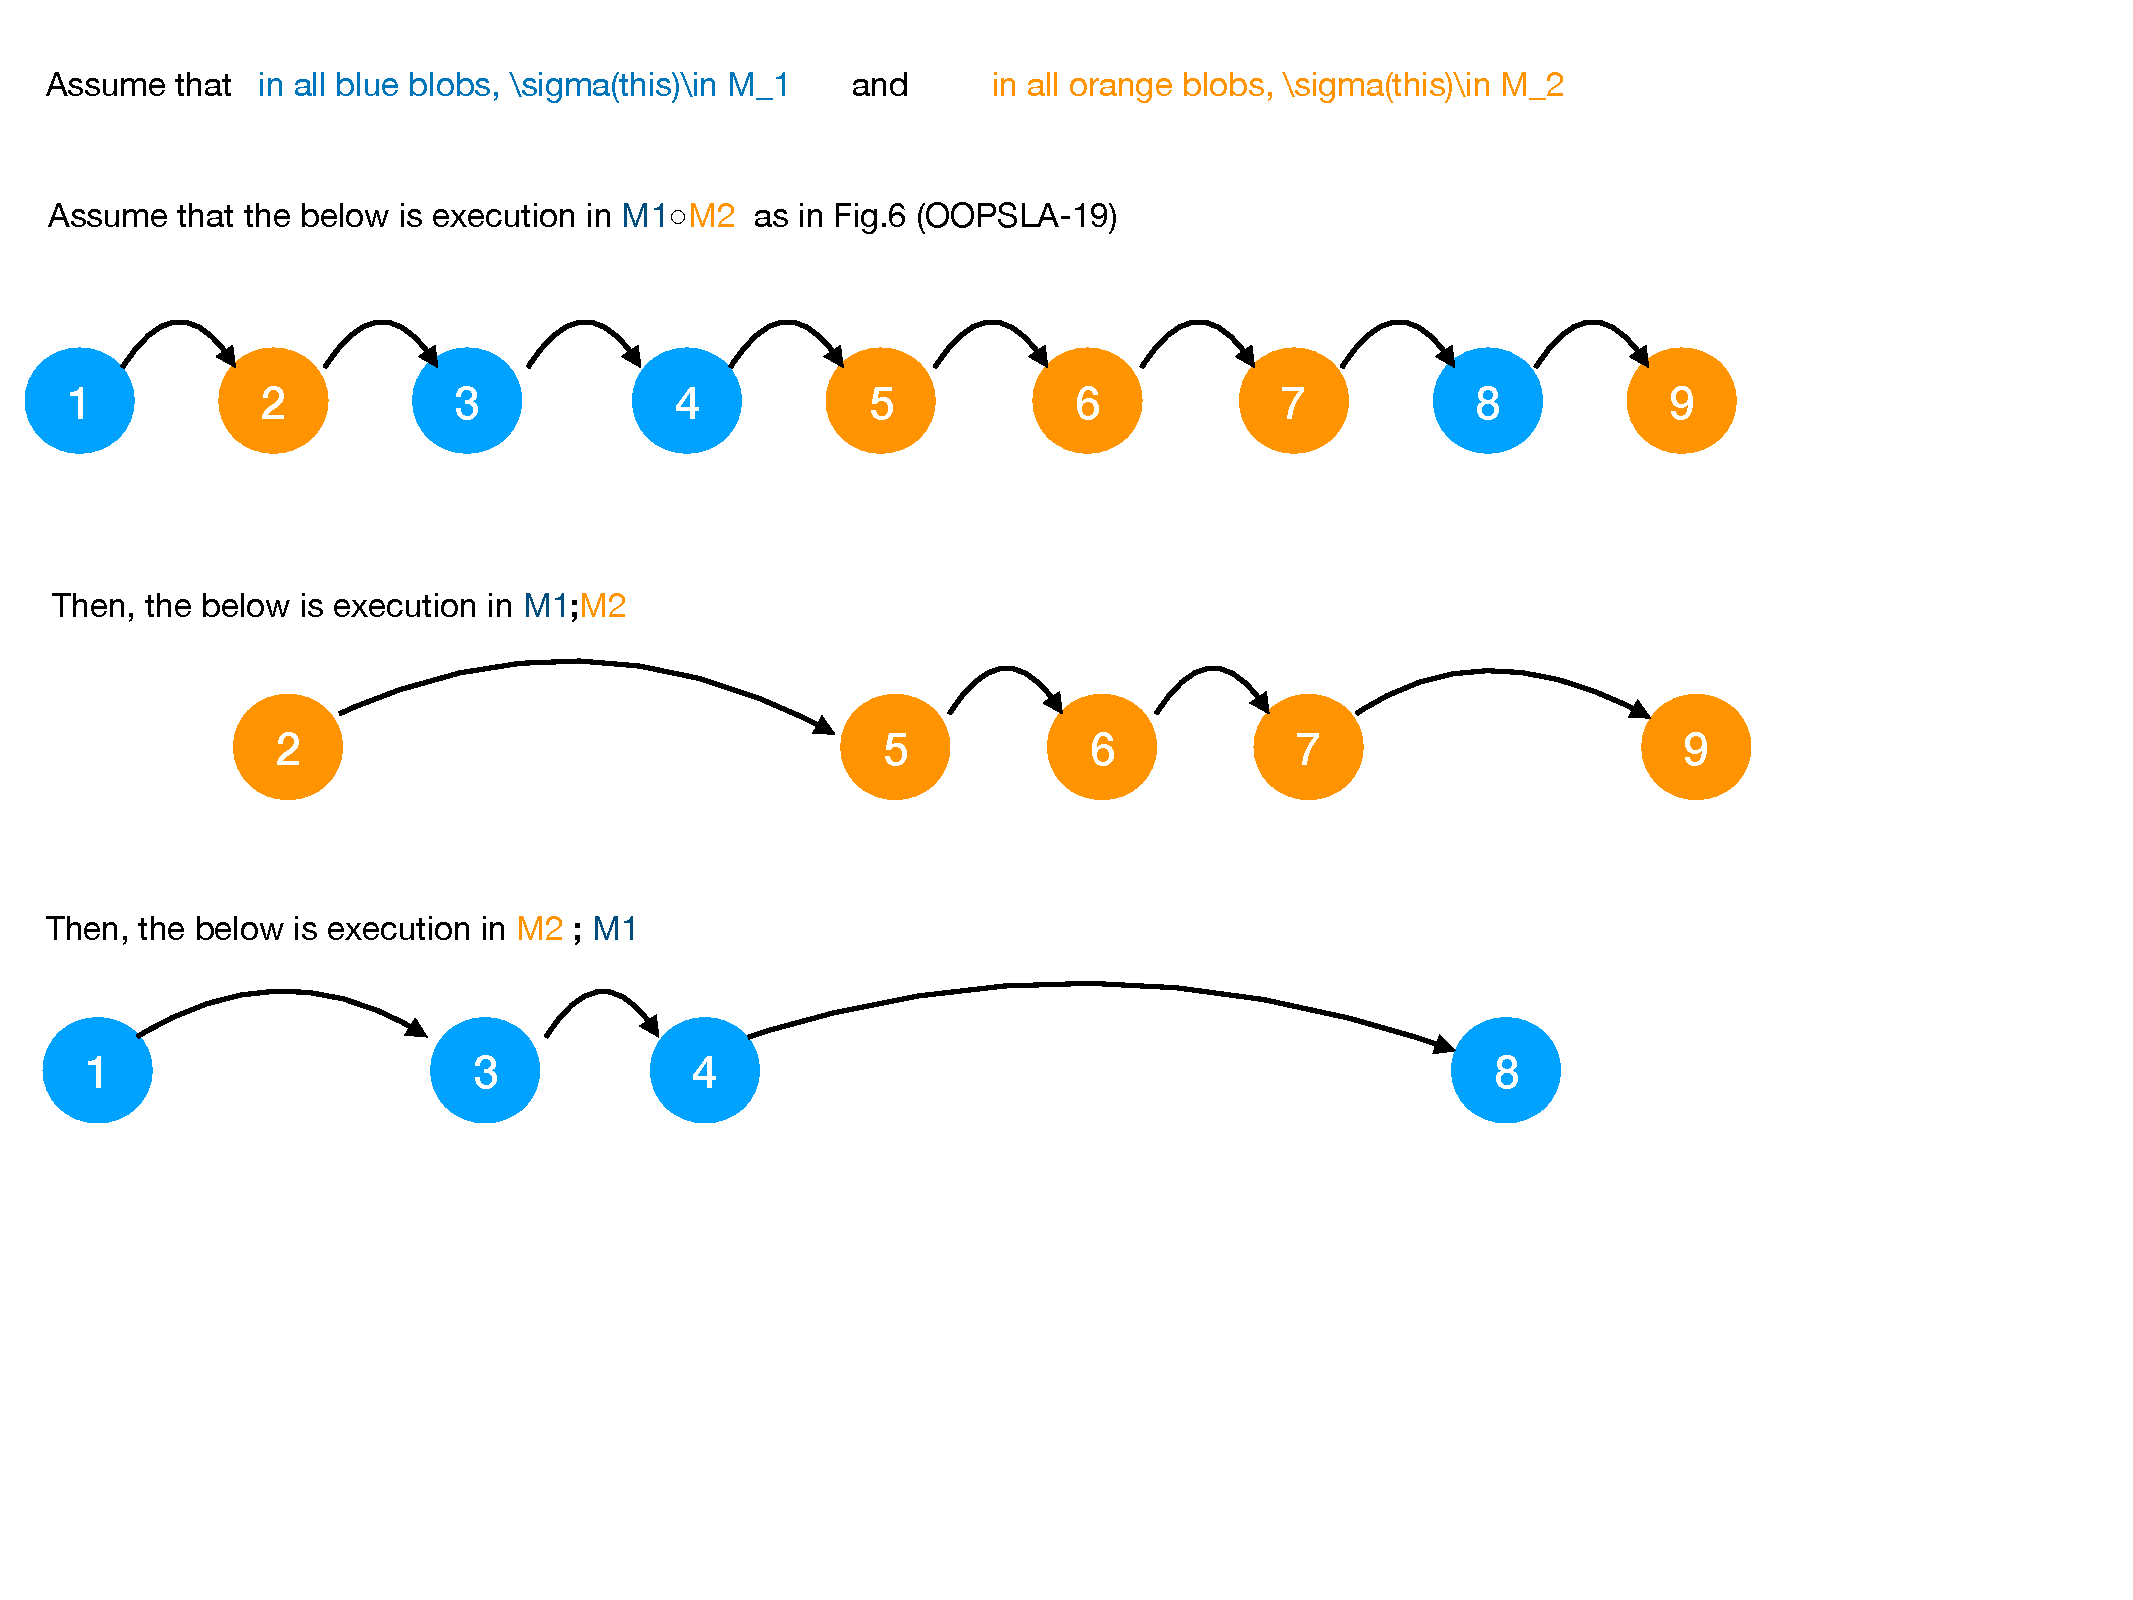
\includegraphics[width=\linewidth]{diagrams/VisibleStates.pdf}
\end{minipage}
  \vspace*{-2.5mm}
  \caption{Illustrating Def. \ref{def:execution:internal:external}}
 \label{fig:VisibleStates}
 \end{figure}
 
In the definition above,  $\ClassOf {\x} {\sigma} $ looks up the class of the object stores at \x\appref{def:interp}.
% If  $n$  has the value $2$, %. In this case the final bullet is trivial and  
%then  there exists a direct, external transition from $\sigma$ to $\sigma'$.  
 For example, for $\sigma_4$ as in Section \ref{sect:chainmail} whose next statement to be executed 
 is  $\prg{a}_2.\prg{deposit}{\prg{(}}\prg{a}_3,\prg{360}{\prg{)}}$,  we would have 
 a sequence of configurations $\sigma_{41}$, ... $\sigma_{4n}$,  $\sigma_{5}$ so that the
  one-module execution gives
 $\M_{BA2}, \sigma_4 \leadsto \sigma_{41} \leadsto \sigma_{42} ... \leadsto \sigma_{4n}   \leadsto \sigma_{5}$.
This would correspond to an atomic evaluation in the two-module execution: \  \
 $\M_{BA2}\mkpair \M', \sigma_4 \ \leadsto \sigma_5$.
 
 We illustrate the definition in Fig. \ref{fig:VisibleStates}.

Two-module execution  is related to % the concept of 
visible states
semantics \cite{MuellerPoetzsch-HeffterLeavens06} as they both filter configurations, with  the difference
that in visible states semantics % \sd{considers all intermediate configurations during execution, but
execution is unfiltered and  configurations are only filtered when it comes to the  consideration 
of class invariants} while {two-module execution filters  execution.
%
The lemma below says  that linking is associative and commutative, and preserves   both one-module and two-module execution.

\begin{lemma}[Properties of linking]
\label{lemma:linking}
 For any modules $\M$,   $\M'$, $\M''$, and $\M'''$ and runtime configurations $\sigma$, and $\sigma'$ we have$:$
 \label{lemma:linking:properties}

 \begin{itemize}
     \item
     $(\M \link \M')\link \M''$ = $\M \link (\M' \link \M'')$  \hspace{1cm} and    \hspace{1cm}   $\M \link \M'$  = $\M' \link\M$.
      \item
      $\M, \sigma \leadsto \sigma'$, and $\M\link \M'$ is defined, \  \ \ \ \  implies\ \ \ \ \   $\M\link \M', \sigma \leadsto \sigma'$.
 \item
 $\M \mkpair \M', \sigma \leadsto \sigma'$   \  \ \ \ \  implies\ \ \ \ \  $(\M\link\M'') \mkpair (\M'\link\M''') ,\sigma \leadsto \sigma'$.  
  \end{itemize}

 \end{lemma}
 
 We can now answer the question as to which runtime configurations are pertinent when judging a module's
adherence to an assertion.
We define as  {\em arising} configurations as those that can be reached by two-module execution, starting from any initial configuration.
An initial configuration has a heap with only one object, of class \prg{Object}, and only one frame, whose continuation may be arbitrary.
 
\begin{definition}[Initial and Arising Configurations] are defined as follows: \label{def:arise}

\begin{itemize}
     \item
   $\Initial {(\psi,\chi)}$, \ \ if \ \ $\psi$ consists of a single frame $\phi$ with $dom(\phi)=\{ \this \}$, and there exists  some address $\alpha$, such that \ \ \    $\interp {\this}{\phi}$=$\alpha$, and \ $dom(\chi)$=$\alpha$,\  and\  
    $\chi(\alpha)=(\prg{Object},\emptyset)$.
 \item
 $\Arising  {\M\mkpair\M'} \ = \ \{ \ \sigma \ \mid \ \exists \sigma_0. \ [\  \Initial{\sigma_0} \  \ \wedge\ \  \M\mkpair\M', \sigma_0 \leadsto^* \sigma \ \ ] \ \ \} $
 \end{itemize}

\end{definition}
